\documentclass[12pt,a4paper]{article}

% Packages
\usepackage[utf8]{inputenc}
\usepackage[T1]{fontenc}
\usepackage{amsmath}
\usepackage{amsfonts}
\usepackage{amssymb}
\usepackage{graphicx}
\usepackage{hyperref}
\usepackage{cite}
\usepackage{url}
\usepackage{float}
\usepackage{booktabs}
\usepackage{multirow}
\usepackage{array}
\usepackage{caption}
\usepackage{xcolor}
\usepackage{geometry}
\geometry{margin=1in}

\title{VIGIL: Vectors of Intelligent Guidance in Long-Reach Rural Healthcare}
\author{Andrew Krikorian}
\date{\today}

\begin{document}

\maketitle

\begin{abstract}
Medical ultrasound procedures require significant expertise and training, creating barriers to access in resource-limited settings and for generalist operators. This paper presents VIGIL (Vectors of Intelligent Guidance in Long-Reach Rural Healthcare), a modular AI-powered assistive technology system designed to provide real-time guidance for medical ultrasound procedures, specifically cardiac left ventricular ejection fraction (LVEF) assessment and lower limb deep vein thrombosis (DVT) detection. VIGIL integrates multiple AI/ML systems from collaborating institutions within a distributed ROS2 architecture, enabling real-time multi-modal feedback through visual guidance, audio instructions, and progress tracking. A key innovation of the system is its comprehensive projection-based guidance system that projects detailed, step-by-step instructions directly onto the patient's body, providing in-situ visual guidance for every phase of the procedure without requiring operators to look away from the patient. At the heart of the system is the VIGIL Agent, an intelligent medical tool orchestrator that coordinates all system components, interprets natural language operator queries, and manages procedure state transitions through contextual understanding. The system's modular design facilitates customization for different procedures and operators, while its usability features support both experienced medical professionals and novices. We describe the system architecture, core components, the VIGIL Agent orchestration framework, the projection-based guidance system, customization capabilities, usability features, and adaptability mechanisms. Additionally, we present the design of ongoing comparative user studies evaluating VIGIL's effectiveness against expert guidance, involving participants ranging from medical students to complete novices. The system demonstrates how AI-powered assistive technologies can address customization, usability, and adaptability challenges in medical procedure guidance, potentially democratizing access to critical diagnostic capabilities in rural and underserved healthcare settings.
\end{abstract}

\textbf{Keywords:} Assistive Technology, Medical Ultrasound, AI-Powered Systems, Human-Computer Interaction, ROS2, Real-Time Guidance

\section{Introduction}

Assistive technologies (ATs) incorporating artificial intelligence (AI) and machine learning (ML) have transformed healthcare delivery, enabling individuals with varying levels of expertise to perform complex medical procedures. However, significant challenges remain in creating systems that are simultaneously customizable to different use cases, usable by operators with diverse experience levels, and adaptable to evolving requirements \cite{frontiers_topic}. Medical ultrasound procedures exemplify these challenges: they require extensive training, real-time decision-making, and precise probe manipulation, yet access to expert guidance is often limited in resource-constrained environments.

\subsection{Problem Statement}

Medical ultrasound procedures, such as cardiac left ventricular ejection fraction (LVEF) assessment and lower limb deep vein thrombosis (DVT) detection, are critical diagnostic tools that traditionally require specialized training. Generalist operators, including medical students and healthcare providers in underserved areas, face significant barriers in performing these procedures effectively. Operators require immediate feedback on probe positioning, image quality, and anatomical landmark identification to successfully complete procedures. Effective guidance systems must provide multi-modal feedback through visual, audio, and in-situ projection channels, adapting to different patient anatomies, operator skill levels, and procedure requirements. The complexity of integrating multiple AI/ML systems—including computer vision for image analysis, pose estimation for patient positioning, and natural language processing for operator interaction—into a cohesive assistive technology presents substantial engineering and design challenges that must be addressed to create truly usable systems.

\subsection{VIGIL System Overview}

VIGIL (Vectors of Intelligent Guidance in Long-Reach Rural Healthcare) addresses these challenges through a modular, distributed architecture that integrates state-of-the-art AI/ML systems from multiple collaborating institutions. The system provides real-time guidance for two primary use cases. The Cardiac Module assists operators in performing LVEF ultrasound procedures through real-time image analysis, anatomical landmark detection, and quality assessment using the University of Pennsylvania's cardiac analysis system. This module processes incoming ultrasound frames to identify key cardiac structures, tracks anatomical landmarks required for ejection fraction measurement, and provides continuous quality feedback to guide operators toward diagnostic-quality images.

The Lower Limb Module guides DVT ultrasound procedures by integrating patient pose estimation from Stevens Institute's SMPL-based system, probe tracking from Cornell University, progress monitoring from Northeastern University, and visual projection guidance from the University of Michigan. This module demonstrates the system's ability to coordinate multiple specialized AI systems, each contributing different capabilities that together provide comprehensive procedural guidance. The module can adaptively select between different probe tracking modalities—including Cornell's specialized tracking, SAM-based segmentation, or hand tracking—based on system availability and performance requirements.

The system's design emphasizes three core principles aligned with the Frontiers research topic themes. Customization is achieved through a modular architecture that allows components to be configured, added, or removed based on specific procedure requirements and operator needs. This enables the system to be tailored for different clinical contexts, from fully-equipped facilities to resource-limited rural settings. Usability is enhanced through multi-modal interfaces including an operator console, real-time visualization displays, speech-to-text, text-to-speech, and visual question answering capabilities that support diverse interaction preferences and operator skill levels. Adaptability is realized through dynamic state management and real-time AI feedback that enable the system to adjust guidance based on operator performance and procedure progress, creating a personalized assistance experience.

\subsection{Contributions}

This paper makes the following contributions:

\begin{enumerate}
    \item A modular ROS2-based architecture for integrating multiple AI/ML systems into a cohesive assistive technology platform
    \item A comprehensive projection-based guidance system that projects step-by-step instructions directly onto the patient's body, providing in-situ visual guidance for every phase of the procedure
    \item A customization framework enabling procedure-specific configurations and external system integration through standardized APIs
    \item Usability features including multi-modal feedback, operator console interfaces, and real-time visualization systems
    \item An adaptability mechanism using state management and temporal synchronization for real-time guidance adjustment
    \item Design and preliminary results from comparative user studies evaluating system effectiveness across operator experience levels
\end{enumerate}

\section{Related Work}

\subsection{AI-Powered Assistive Technologies in Healthcare}

AI-powered assistive technologies have shown promise in various healthcare applications, from smart wheelchairs to augmentative communication devices \cite{assistive_tech_review}. In medical imaging, AI systems have primarily focused on automated image interpretation rather than real-time procedural guidance \cite{medical_ai_review}. However, recent work has explored AI-assisted surgical guidance \cite{surgical_guidance} and telemedicine applications \cite{telemedicine_ai}, demonstrating the potential for AI to enhance operator capabilities rather than replace them.

\subsection{Medical Ultrasound Guidance Systems}

Existing ultrasound guidance systems have typically focused on specific aspects such as probe tracking \cite{probe_tracking}, image quality assessment \cite{image_quality}, or anatomical landmark detection \cite{landmark_detection}. Few systems integrate multiple guidance modalities into a unified platform. Commercial systems often require proprietary hardware and lack the modularity needed for customization to different procedures or operator skill levels.

\subsection{Modular Robotics and ROS Architectures}

The Robot Operating System (ROS) and its successor ROS2 have become standard frameworks for distributed robotic systems \cite{ros2_paper}. ROS2's distributed architecture, quality of service (QoS) policies, and language-agnostic design make it well-suited for integrating heterogeneous AI/ML systems. However, applying ROS2 architectures to assistive technologies in healthcare requires careful consideration of real-time requirements, data privacy, and human-computer interaction design.

\subsection{Multi-Modal Human-Computer Interaction in Medical Contexts}

Effective assistive technologies in medical settings require multi-modal interaction capabilities. Research in medical HCI has explored voice interfaces \cite{voice_hci} and augmented reality guidance \cite{ar_guidance}. However, integrating these modalities into a cohesive system that adapts to operator needs and provides comprehensive step-by-step guidance directly on the patient remains challenging.

\section{System Architecture}

The VIGIL system architecture integrates multiple specialized components from collaborating institutions within a distributed ROS2 framework. Figure~\ref{fig:system_architecture} illustrates the overall system architecture, showing data flows between sensors, processing modules, the VIGIL Agent orchestrator, and output systems. The architecture demonstrates the modular design where components from different institutions (University of Pennsylvania, University of Rochester, University of Michigan, Cornell University, Stevens Institute, Northeastern University, and California State University) integrate seamlessly through standardized ROS2 message types and the VIGIL Agent's orchestration layer.

\begin{figure}[h]
\centering
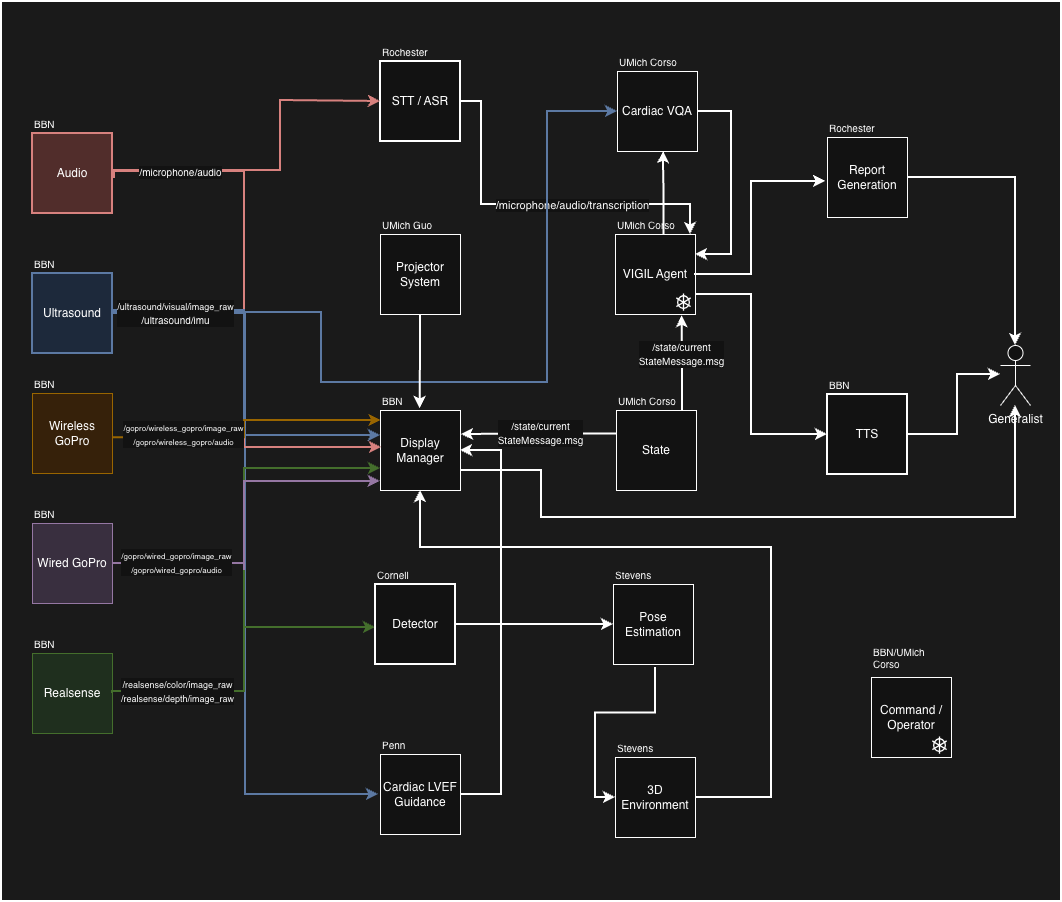
\includegraphics[width=0.9\textwidth]{assets/ros2_communcation_system.png}
\caption{VIGIL System Architecture showing data flows between sensors, processing modules, the VIGIL Agent orchestrator, and output systems. Components are labeled with their originating institutions.}
\label{fig:system_architecture}
\end{figure}

\subsection{Overall Design Philosophy}

VIGIL employs a distributed ROS2 architecture that enables modular component design and seamless integration of external AI/ML systems. The architecture follows several key design principles that together create a flexible, maintainable, and extensible system. Each functional component operates as an independent ROS2 node, enabling components to be added, removed, or modified without affecting the entire system. This modularity is essential for a system that must integrate contributions from multiple collaborating institutions, each with different development timelines and update schedules.

Components communicate through standardized message types and topics, reducing dependencies between modules and enabling parallel development. This decoupling ensures that changes to one component's internal implementation do not require modifications to other components, as long as the message interfaces remain consistent. The UniversityAPI abstraction layer provides a consistent interface for integrating external systems from different institutions, allowing each university's system to be wrapped in a standardized API while preserving their unique internal implementations. ROS2's quality of service policies and temporal synchronization utilities ensure timely data flow for real-time guidance, which is critical for medical procedures where delayed feedback could impact procedure quality or operator confidence.

\subsection{Core Components}

\subsubsection{Cardiac Module}

The cardiac module provides comprehensive guidance for LVEF ultrasound procedures through deep integration with the University of Pennsylvania's cardiac analysis system. This module processes incoming ultrasound frames in real-time to assess image quality and identify anatomical structures, enabling operators to understand whether their current probe positioning is capturing diagnostically useful views. The system continuously analyzes each frame to detect key cardiac landmarks required for LVEF measurement, including the left ventricular walls, mitral valve, and apex. As operators manipulate the probe, the system provides real-time estimates of left ventricular ejection fraction, giving immediate feedback on whether the current view is suitable for measurement.

The module publishes annotated ultrasound images with overlays indicating detected landmarks, quality metrics, and guidance information. These annotations help operators understand what the system is detecting and guide them toward optimal probe positioning. The visual feedback includes color-coded indicators for image quality, highlighted anatomical structures, and directional guidance for probe movement. Additionally, the module generates structured reports containing procedure data for documentation, including timestamps, quality metrics, detected landmarks, and LVEF estimates. The cardiac module subscribes to ultrasound image streams and IMU (Inertial Measurement Unit) data from the probe, processes frames through the UPenn system API, and publishes guidance information to display and reporting components throughout the ROS2 network.

Performance evaluation of the cardiac module demonstrates high accuracy in landmark detection, with an average mean Euclidean distance error of 2.47±1.29 pixels across all visible landmarks on the EchoNet Dynamic test set. Key landmarks critical for LVEF measurement show precise localization: left ventricular apex (3.18 ± 5.84 pixels), mitral valve (3.60 ± 9.81 pixels), right ventricle (2.33 ± 1.28 pixels), and tricuspid valve (2.37 ± 2.30 pixels). The transducer guidance network achieves mean rotation prediction errors of 5.3-5.5° on validation data and 7.0-7.2° on held-out subjects, with 90th percentile errors of approximately 10° and 18° respectively, indicating strong alignment for most frames. The system processes frames at an average rate of 14 frames per second, enabling real-time guidance during procedures. Automated LVEF predictions average 50.7\% ± 4.8\%, compared to expert-estimated LVEF of 59.5\% ± 6.0\%, demonstrating the system's capability to provide quantitative cardiac function assessment.

\subsubsection{Lower Limb Module}

The lower limb module guides DVT ultrasound procedures by integrating multiple specialized systems that each contribute unique capabilities to the overall guidance framework. The module uses Stevens Institute's SMPL-based system to estimate and render 3D patient pose from camera data, creating a real-time model of the patient's body position that enables context-aware guidance. This pose estimation allows the system to understand the patient's orientation and limb positioning, which is critical for guiding operators to the correct anatomical regions for DVT scanning.

Probe tracking is accomplished through integration with Cornell University's specialized probe tracking system, which uses computer vision to identify and track the ultrasound probe's position and orientation in 3D space. The module includes fallback options including SAM-based segmentation and hand tracking, demonstrating the system's robustness and adaptability. When Cornell's tracking system is unavailable or encounters difficulties, the system can seamlessly switch to alternative tracking modalities, ensuring continuous guidance capability. Progress tracking is monitored using Northeastern University's progress tracking system, which analyzes the scanning pattern and coverage to determine how much of the required anatomical region has been examined. The system uses a causal Temporal Convolutional Network (TCN) architecture that processes multimodal features from both RealSense camera and ultrasound data to predict vein type and procedure progress in real-time. Evaluation on held-out data demonstrates vein segmentation accuracy of 67.6\% on validation sets, with progress estimation mean absolute error of 14.1\%. The system operates with low computational requirements (under 1 GB GPU VRAM) and provides continuous feedback such as "you've scanned 60\% of the required area" or "move the probe slightly superior to cover the remaining region," enabling operators to understand procedure completion status throughout the scan.

Visual guidance is provided through the University of Michigan's comprehensive projection system, which represents a key innovation in procedural guidance. The projection system projects detailed, step-by-step instructions directly onto the patient's body, providing in-situ visual guidance for every phase of the procedure. This system goes beyond simple probe placement indicators to provide comprehensive procedural guidance including patient alignment instructions, target area indicators that dynamically update based on patient pose, reference lines showing anatomical landmarks, scan path visualizations, progress indicators, and real-time quality feedback. The projection system uses marker-based calibration to align with the physical world and joint-based patient alignment to dynamically adjust guidance elements based on real-time patient pose estimation. This enables the system to project guidance that follows the patient's body movements, ensuring that instructions remain accurate even as the patient shifts position. The system provides procedure-specific guidance: for cardiac procedures, it projects the position of the 5th intercostal space, midclavicular line, and LVEF indicators; for lower limb procedures, it projects guidance lines from hip to knee with color-coded regions indicating scanned areas (green for good quality, white for next area, yellow for unscanned, red for poor quality). This comprehensive projection-based guidance eliminates the need for operators to look away from the patient to check screens, reducing context switching and facilitating shared understanding between operator and patient. The module also coordinates with California State University's DVT-specific analysis system, which provides specialized image analysis for deep vein thrombosis detection. The lower limb module demonstrates the system's modularity by allowing different probe tracking modes to be selected based on availability and performance requirements, enabling the system to adapt to different hardware configurations and environmental conditions.

\subsection{The VIGIL Agent: Intelligent Medical Tool Orchestration}

At the heart of the VIGIL system is the VIGIL Agent, an intelligent medical tool orchestrator that functions as a "medical Jarvis"—an AI-powered coordinator that understands operator intent, manages system state, and orchestrates interactions between all components. The VIGIL Agent serves as the central intelligence layer that makes the distributed system feel like a unified, responsive assistant rather than a collection of independent tools.

The VIGIL Agent operates by continuously monitoring multiple data streams from across the system. It receives speech-to-text transcriptions from the operator, processes incoming ultrasound frames, and tracks the current procedure state. When an operator speaks, the agent uses natural language understanding to determine the operator's intent, whether they are asking a question about the procedure, requesting system information, or indicating that they are ready to proceed to the next step. The agent employs a large language model (LLM) to interpret operator utterances in the context of the current procedure state, enabling it to understand implicit requests and contextual cues that would be difficult to handle with rule-based systems.

One of the agent's key capabilities is intelligent tool orchestration. When an operator asks a question, the agent determines which specialized system should handle the query. For questions about visual content in ultrasound images, the agent routes the query to the Visual Question Answering (VQA) system. For general medical questions, it routes to the General Medical LLM. For state management requests, it processes them directly using contextual understanding of the procedure workflow. This tool selection is performed dynamically based on the content and context of each query, rather than requiring operators to specify which system to use.

The agent also manages procedure state transitions through natural language understanding. Operators can indicate readiness to proceed by saying things like "I've finished aligning the patient" or "the probe is in position," and the agent uses contextual trigger detection to recognize these implicit state transition requests. The agent maintains awareness of the current procedure state and valid state transitions, enabling it to understand when operators are ready to move to the next phase of the procedure. This natural language state management reduces the cognitive load on operators, who can communicate naturally rather than learning specific commands or menu structures.

The VIGIL Agent's architecture enables it to coordinate between multiple specialized systems seamlessly. It maintains queues for incoming frames and operator prompts, ensuring that it always has access to the most recent visual and audio context when processing queries. When the agent determines that a question requires visual analysis, it captures the current ultrasound frame at the moment the question is asked, ensuring that the VQA system receives the relevant visual context. This temporal alignment between operator queries and visual data is critical for providing accurate, contextually relevant responses.

The agent's orchestration capabilities extend beyond simple routing. It can coordinate multi-step interactions, such as when an operator's question requires both visual analysis and general medical knowledge. The agent manages the flow of information between systems, ensuring that responses are synthesized and presented to the operator in a coherent manner. This orchestration makes the complex underlying system architecture transparent to operators, who interact with what feels like a single, intelligent assistant rather than multiple disconnected tools.

The VIGIL Agent demonstrates how AI-powered orchestration can address the integration complexity challenge in assistive technologies. By providing a unified interface that understands operator intent and coordinates specialized systems, the agent enables operators to focus on the medical procedure rather than learning how to interact with multiple tools. This design philosophy—hiding complexity behind intelligent orchestration—is essential for creating truly usable assistive technologies that can be effectively used by operators with varying levels of technical expertise.

\subsubsection{VIGIL Agent Performance Evaluation}

Comprehensive performance evaluation of the VIGIL Agent has been conducted to assess its effectiveness in tool routing and response generation. The agent's performance is critical because all downstream behavior, including state management, tool use, and guidance generation, relies on accurate interpretation of operator intent. The evaluation focused on two key metrics: time to response (TTR) or time to guidance (TTG), and tool calling accuracy.

Time to response measurements evaluated different system prompt configurations to optimize latency while maintaining accuracy. Table~\ref{tab:ttr_performance} shows the performance of different prompt configurations using the Qwen2.5 model. The evaluation revealed that embedding state management within the prompt rather than using a separate tool call substantially reduces latency. The SimplestToolsPrompt configuration, which omits the state tool and uses minimal formatting, achieved an average TTR/TTG of 4.5 seconds, representing a 51\% reduction compared to configurations with separate state management tools. This optimization is critical for real-time medical procedures where delayed feedback could impact operator confidence and procedure quality.

\begin{table}[h]
\centering
\caption{Time to Response/Time to Guidance (TTR/TTG) Performance for Different Prompt Configurations}
\label{tab:ttr_performance}
\begin{tabular}{lcc}
\toprule
\textbf{System Prompt} & \textbf{Model} & \textbf{Avg. TTR/TTG (seconds)} \\
\midrule
OriginalPrompt & Qwen2.5 & 27.3 \\
OriginalToolsPrompt & Qwen2.5 & 42.1 \\
ReducedToolsPrompt & Qwen2.5 & 18.7 \\
SimpleToolsPrompt & Qwen2.5 & 8.7 \\
SimplestToolsPrompt & Qwen2.5 & 4.5 \\
\bottomrule
\end{tabular}
\end{table}

Tool calling accuracy evaluation assessed the agent's ability to correctly route operator queries to appropriate tools. The evaluation tested three output format configurations (JSON, YAML, and TEXT) across 70 standardized test queries covering visual question answering (VQA), general medical question answering (GMQA), and queries requiring no tool. Table~\ref{tab:tool_calling_performance} presents the comprehensive performance results. The JSON format achieved the highest accuracy at 97.1\% (68/70 correct classifications), while maintaining consistent performance characteristics. The TEXT format, while achieving 40\% faster response times (0.237s vs 0.323s) and 41\% fewer output tokens, showed slightly lower accuracy at 94.3\%. This trade-off between accuracy and efficiency is important for deployment decisions, with JSON format recommended for production use due to its superior accuracy in medical applications where routing errors could impact clinical workflows.

\begin{table}[h]
\centering
\caption{VIGIL Agent Tool Calling Performance Comparison}
\label{tab:tool_calling_performance}
\begin{tabular}{lccc}
\toprule
\textbf{Metric} & \textbf{JSON Format} & \textbf{YAML Format} & \textbf{TEXT Format} \\
\midrule
Accuracy & 97.1\% (68/70) & 95.7\% (67/70) & 94.3\% (66/70) \\
Avg. Response Time & 0.323s & 0.289s & 0.237s \\
Avg. Tokens Generated & 8.6 & 7.1 & 5.1 \\
Throughput & 26.3 tokens/sec & 23.9 tokens/sec & 20.2 tokens/sec \\
\bottomrule
\end{tabular}
\end{table}

The evaluation demonstrated strong performance across all query categories. VQA queries (visual interpretation and scanning technique questions) showed high accuracy in identifying visual context keywords and routing to the appropriate tool. GMQA queries (general medical knowledge questions) were effectively discriminated from VQA queries, with accurate identification of medical knowledge questions without visual components. No-tool queries (external search requests and casual conversation) were effectively filtered, with good recognition of temporal indicators and external information requests. The consistently high accuracy (exceeding 94\%) across all formats validates the effectiveness of the underlying prompt design and decision logic, independent of output format choice.

\subsection{Supporting Systems}

\subsubsection{Speech Processing}

The system includes bidirectional speech processing capabilities that enable natural language interaction. Speech-to-text functionality integrates the University of Rochester's speech recognition system, enabling operators to provide voice commands and ask questions without needing to use their hands to interact with the system. The system uses OpenAI Whisper Medium model, selected after comprehensive evaluation comparing five model variants (Tiny through Large v3) across diverse speakers. Whisper Medium achieved a Mean Opinion Score (MOS) of 7.4 for "VIGIL" keyword detection stability, outperforming larger models (Large v3 Turbo: 6.8 MOS) which showed higher hallucination rates. The system employs prompt engineering to improve recognition of the specialized "VIGIL" trigger keyword, which is critical for state transitions and agent activation. This hands-free interaction is particularly valuable during medical procedures where operators need to maintain contact with the patient or manipulate the ultrasound probe. The system continuously processes operator speech, converting spoken words into text that can be understood by the VIGIL Agent and other system components.

Text-to-speech capabilities use Piper voice synthesis to provide audio feedback and instructions to operators. Performance evaluation demonstrates perfect speech accuracy with no errors or deviations observed during both controlled tests and live demonstrations. For typical sentence-length inputs from the VQA system, total execution time averages approximately 0.5 seconds, providing fast and natural interaction. The system uses a dual-thread design that enables generation of new speech while simultaneously playing previously generated audio, improving overall responsiveness. This audio feedback can include guidance instructions, quality alerts, progress updates, and responses to operator questions. The system supports multiple voice models (e.g., en-US-kusal-medium), allowing customization based on operator preferences or clinical context. The combination of speech-to-text and text-to-speech creates a conversational interface that enables operators to interact with the system naturally, asking questions and receiving spoken responses while performing procedures.

\subsubsection{Visual Question Answering}

The University of Michigan VQA system enables operators to ask natural language questions about the procedure, ultrasound images, or system state, receiving AI-generated responses based on visual and contextual information. When an operator asks a question about what they are seeing in an ultrasound image, the VIGIL Agent routes the query to the VQA system along with the current ultrasound frame. The VQA system uses vision-language models to analyze both the visual content of the image and the natural language question, generating responses that are specific to what the operator is currently viewing. Evaluation on a held-out test set of 1,000 ultrasound images demonstrates strong performance: Exact Match of 48.18, F1 score of 44.95, Precision of 50.03, and Recall of 42.86. For binary clinical decisions (yes/no questions about chamber visibility, EF measurability, and image quality), the system achieves 90.59\% accuracy, which is particularly relevant since most operator questions are binary assessments. The model is trained on approximately 15,000 ultrasound images with expert-written and GPT-4o-generated question-answer pairs, ensuring diverse linguistic variation to reduce language-prior bias. This capability is particularly valuable for training and education, as operators can ask questions like "Is this a good view of the left ventricle?" or "What landmark am I looking at?" and receive immediate, contextually relevant answers.

\subsubsection{Display and Visualization}

The display system provides comprehensive real-time visualization through multiple specialized display nodes, each optimized for different aspects of the procedure. The Debug Display provides comprehensive system monitoring and debugging capabilities, showing the status of all components, message flow, and system health metrics. This display is primarily used during development and troubleshooting but can also be valuable for understanding system behavior during procedures.

The Guidance Display provides procedure-specific guidance visualization, showing annotated ultrasound images, quality metrics, and directional guidance for probe movement. This is the primary interface that operators use during procedures, providing the visual feedback they need to perform scans effectively. The Pose Display renders 3D patient pose with annotations, showing the estimated patient position and orientation along with procedure-specific markers indicating target scan regions. The Visualization Display provides real-time data visualization, including graphs of quality metrics over time, progress indicators, and other temporal data that helps operators understand procedure progress. The display system supports both cardiac and lower limb procedure layouts, with configurable widgets and windows that can be arranged based on operator preferences and procedure requirements.

\subsubsection{State Management}

The state management system tracks procedure state transitions and coordinates component behavior based on current state, enabling context-aware guidance and adaptive system behavior. The system defines multiple procedure states such as patient alignment, gross probe guidance, and fine probe guidance, each representing a distinct phase of the procedure. Components throughout the system subscribe to state updates and adjust their behavior accordingly. For example, when the system transitions to the "fine probe guidance" state, the guidance algorithms may switch to more precise feedback modes, and the display may show different visualizations optimized for fine positioning. The VIGIL Agent uses state information to provide contextually appropriate responses and to understand when operators are indicating readiness to proceed to the next phase.

\subsubsection{Command and Control}

The vigil\_c2 (VIGIL Command and Control) package provides operator interfaces for system control, complementing the natural language interaction enabled by the VIGIL Agent. The Operator Console provides a curses-based terminal interface for component-specific commands, enabling operators to access advanced features and system controls through keyboard input. This interface uses a two-level menu hierarchy, with a main menu for component selection and sub-menus for component-specific commands. The Qt6 Widget provides a graphical interface for system control that can be integrated into the display system or run standalone. Both interfaces use a JSON-based menu configuration system that enables customizable command interfaces, allowing the system to be configured for different procedures and operator preferences. While the VIGIL Agent handles most operator interactions through natural language, the command and control interfaces provide direct access to system functions for operators who prefer explicit control or need to access advanced features.

\subsection{Communication Framework}

\subsubsection{Custom Message Types}

VIGIL defines over 20 custom ROS2 message types in the vigil\_msgs package, creating a standardized communication protocol that enables components to exchange data efficiently. The \texttt{FrameMessage} type encapsulates compressed image data with metadata including timestamps and source information, enabling efficient transmission of ultrasound frames across the network. \texttt{AnnotatedUltrasound} messages contain ultrasound images with annotations and guidance overlays, allowing display components to render annotated views without needing to recompute annotations. \texttt{PatientPose} and \texttt{PatientPoseRaw} messages carry 3D pose estimation data from the Stevens Institute system, enabling components throughout the system to understand patient positioning. \texttt{ProbeTipPrediction} messages contain probe position and orientation estimates from tracking systems, providing the spatial information needed for guidance algorithms. \texttt{ProgressTracking} messages carry procedure progress metrics, enabling the system to provide operators with feedback on scan coverage and completion. \texttt{ProjectionGuidance} messages contain visual guidance instructions for the projection system, specifying where and how to display guidance indicators. \texttt{VigilC2Message} messages enable command and control functionality, allowing the operator console and VIGIL Agent to send commands to components. \texttt{VQAMessage} messages encapsulate visual question answering queries and responses, enabling the VIGIL Agent to route questions to the VQA system and receive answers.

\subsubsection{Communication Patterns}

The system employs multiple communication patterns optimized for different types of interactions. The publisher-subscriber pattern serves as the primary mechanism for data distribution, used for streaming images, poses, guidance information, and other high-frequency data. This asynchronous pattern enables components to receive updates without blocking, which is essential for real-time performance. Components can subscribe to topics of interest and receive updates as they become available, enabling loose coupling between data producers and consumers.

The service-client pattern is used for synchronous operations such as operator input handling and component queries. When an operator uses the console to send a command to a component, the console acts as a client making a service call to the component's service. This synchronous pattern ensures that commands are received and processed before the operator interface continues, providing immediate feedback on command execution. ROS2 message delivery latency for VIGIL's use cases is on the order of 3-5 milliseconds, with potential for optimization to tens of microseconds using shared memory transport. However, temporal synchronization presents a more significant challenge: evaluation of multi-camera data streams revealed maximum time differences of up to 0.44 seconds between camera pairs, with average differences ranging from 0.11 to 0.25 seconds depending on camera configuration. To address this, the system implements a TemporalStreamAligner utility that aligns data streams with different timestamps, ensuring that when the VIGIL Agent processes a question about a specific ultrasound frame, it uses the frame that was captured at the time the question was asked, rather than the most recent frame. This temporal alignment is critical for providing accurate, contextually relevant responses and for multi-modal processing that requires synchronized data from multiple sensors.

\section{Customization Framework}

\subsection{Modular Design Principles}

VIGIL's customization capabilities stem from its modular architecture, where each component can be independently configured, enabled, or disabled based on procedure requirements. This modularity enables the system to be tailored for different clinical contexts, from fully-equipped facilities with all components available to resource-limited settings where only essential components are deployed. The system supports multiple configuration levels that work together to provide flexible customization.

Launch scripts provide procedure-specific launch configurations, such as \texttt{launch\_cardiac.sh} and \texttt{launch\_lower\_limb.sh}, which start only the components needed for each procedure type. These scripts handle the complexity of starting multiple ROS2 nodes in the correct order with appropriate parameters, making it straightforward to launch the system for a specific use case. Configuration files in INI format specify system parameters, model paths, and component settings, enabling fine-grained control over system behavior without modifying code. Runtime parameters through ROS2's parameter system enable dynamic configuration without system restart, allowing operators or the VIGIL Agent to adjust system behavior during procedures based on real-time conditions.

\subsection{External System Integration}

\subsubsection{UniversityAPI Abstraction}

The \texttt{UniversityAPI} abstract base class provides a standardized interface for integrating external systems:

\begin{verbatim}
class UniversityAPI(ABC):
    @abstractmethod
    def run(self, *args, **kwargs)
    @abstractmethod
    def stop(self, *args, **kwargs)
    @abstractmethod
    def status(self, *args, **kwargs)
    @abstractmethod
    def process_command(self, msg: VigilC2Message)
\end{verbatim}

This abstraction enables different university systems to be integrated while maintaining consistent interfaces for the VIGIL framework.

\subsubsection{Integration Examples}

The UniversityAPI abstraction has been successfully used to integrate systems from multiple collaborating institutions. The \texttt{UPennSystemAPI} wraps the University of Pennsylvania's cardiac analysis system, handling the complexities of image processing, landmark detection, and LVEF prediction while presenting a clean interface to the cardiac module. The \texttt{CSUSystemAPI} integrates California State University's DVT analysis system, enabling the lower limb module to access specialized DVT detection algorithms. The \texttt{RochesterAudioAPI} interfaces with the University of Rochester's speech recognition system, providing speech-to-text capabilities to the VIGIL Agent and other components. The \texttt{UMichVQAAPI} and \texttt{UMichProjectionAPI} connect University of Michigan's VQA and comprehensive projection systems. The projection API enables the system's innovative in-situ guidance capabilities, projecting detailed step-by-step instructions directly onto the patient's body for every phase of the procedure. Each API implementation handles the specific requirements, data formats, and communication protocols of its underlying system while presenting a uniform interface to VIGIL components, enabling seamless integration of diverse systems developed by different teams.

\subsection{Configuration Management}

\subsubsection{System Configuration}

The \texttt{config.ini} file specifies system-wide parameters that control system behavior across all components. This includes model weight file paths, which tell components where to find the pre-trained AI models they need to function. The configuration file also specifies voice synthesis model selection for the text-to-speech system, allowing customization of the audio feedback voice based on operator preferences or clinical context. Component-specific settings enable fine-tuning of individual component behavior, such as adjusting sensitivity thresholds or selecting between different algorithm options. Display and visualization preferences control how information is presented to operators, including color schemes, window layouts, and information density.

\subsubsection{Menu Configuration}

The operator console menu system is configured via JSON, enabling flexible customization of the command interface. The configuration supports component-specific command menus, allowing each component to define its own set of commands that operators can access. Command and control (C2) topic definitions enable the menu system to publish commands to components through ROS2 topics, supporting both component-specific commands and system-wide commands. The configuration includes user prompts and parameter collection specifications, enabling commands that require additional input from operators. The menu system can dynamically generate menus based on available components, ensuring that operators only see commands for components that are currently active in the system.

\subsection{Use Case Adaptability}

The system's modularity enables rapid adaptation to different procedures through multiple mechanisms. Component selection ensures that only required components are launched for each procedure type, reducing resource usage and system complexity. For cardiac procedures, the system launches the cardiac module, UPenn system integration, and cardiac-specific display layouts, while lower limb procedures launch the lower limb module, pose estimation, probe tracking, and DVT-specific components. Procedure-specific layouts in the display system are tailored to cardiac versus lower limb procedures, showing relevant visualizations and information for each procedure type. Adaptive guidance algorithms adjust their behavior based on procedure type and operator experience level, providing more detailed guidance for novices and more concise feedback for experienced operators. This adaptability enables the same underlying system architecture to support diverse use cases while maintaining optimal performance and usability for each specific application.

\section{Usability Features}

\subsection{Operator Console}

The operator console provides two interface options for system control:

\subsubsection{Curses-Based Terminal Interface}

A terminal-based menu system enables keyboard-driven control:

\begin{itemize}
    \item Two-level menu hierarchy: main menu for component selection, sub-menus for component-specific commands
    \item Single-character command activation with optional parameter input
    \item Real-time feedback on command execution status
    \item Component-specific input handling through ROS2 services
\end{itemize}

\subsubsection{Qt6 Widget Interface}

A graphical widget interface provides:

\begin{itemize}
    \item Visual menu representation
    \item Integration with the debug display application
    \item Standalone execution capability
    \item Consistent menu configuration with terminal interface
\end{itemize}

\subsection{Display System}

The display system provides real-time visualization through specialized nodes:

\begin{itemize}
    \item \textbf{Annotated Ultrasound Images}: Real-time overlay of landmarks, quality metrics, and guidance information
    \item \textbf{3D Patient Pose Rendering}: Visualization of estimated patient pose with procedure-specific annotations
    \item \textbf{Guidance Overlays}: Visual indicators for probe placement, scan paths, and target regions
    \item \textbf{Progress Visualization}: Real-time progress tracking displays
    \item \textbf{Multi-Window Support}: Configurable window layouts for different procedure types
\end{itemize}

\subsection{Multi-Modal Feedback}

\subsubsection{Projection-Based Visual Guidance}

The projection system represents a key innovation in procedural guidance, providing comprehensive, step-by-step visual instructions projected directly onto the patient's body. This in-situ guidance system eliminates the need for operators to look away from the patient to check screens, reducing context switching and enabling operators to maintain focus on the procedure while receiving detailed guidance.

The projection system provides comprehensive guidance for every step of the procedure. For patient alignment, the system projects body contour images that show the expected patient posture and position, helping operators ensure proper patient positioning before beginning the scan. Target area indicators are projected as rectangular boxes over the patient's body, dynamically updating based on real-time patient pose estimation. For cardiac procedures, the system projects the position of the 5th intercostal space with text descriptions, while for lower limb procedures, it projects target areas around the hip and along the leg. These indicators update in real-time as the patient moves, ensuring guidance remains accurate throughout the procedure.

Reference and guidance lines provide anatomical landmarks and scan paths. For cardiac procedures, the midclavicular line is projected to guide probe placement. For lower limb procedures, guidance lines extend from hip to knee with color-coded rectangular boxes indicating different regions: green for successfully scanned areas with good quality, white for the next area to be scanned, yellow for unscanned areas, and red for scanned areas with poor quality results. Extended lines above each box ensure guidance remains visible even when the box is covered by the operator's hand or probe.

The system projects probe location indicators as red dots that track the probe's position in real-time, enabling operators to see exactly where the probe is relative to target areas. Progress indicators show procedure completion status, with progress bars and step descriptions projected above the patient's head for cardiac procedures. Quality feedback is integrated throughout, with projected elements changing color based on real-time image quality assessment. For cardiac procedures, LVEF indicators are projected as rectangles with numeric percentages that update color based on ejection fraction results.

The projection system uses sophisticated calibration and alignment mechanisms. Marker-based calibration uses ArUco markers placed at the corners of the desired projection region to establish precise alignment between the projection and physical world. Joint-based patient alignment uses real-time 2D joint coordinates from pose estimation to dynamically calculate projection areas, with specific landmarks (e.g., left clavicle, left hip, left knee) serving as anchor points. This enables the projection to follow patient movements in real-time, maintaining accurate guidance even as the patient shifts position.

The comprehensive nature of the projection system enables it to guide operators through every step of the procedure, from initial patient alignment through probe placement, scanning trajectories, and quality assessment. This eliminates the need for operators to memorize procedure steps or refer to external documentation, as all necessary guidance is projected directly onto the patient in real-time.

\subsubsection{Audio Feedback}

Text-to-speech capabilities enable spoken instructions and guidance, allowing operators to receive feedback without needing to look at a display. The system provides quality alerts and warnings when image quality drops below acceptable thresholds or when the probe moves outside the optimal scanning region. Progress announcements inform operators of procedure completion status, such as "you have scanned 75\% of the required area" or "proceeding to fine guidance phase." Error notifications alert operators to issues such as probe disconnection or system component failures, enabling rapid response to problems.

\subsubsection{Speech Input}

Speech-to-text integration allows voice commands for system control, enabling operators to interact with the system without using their hands. Operators can ask natural language questions via the VQA system, receiving spoken responses that help them understand what they are seeing or what actions to take next. This hands-free operation is particularly valuable during medical procedures where operators need to maintain contact with the patient or manipulate the ultrasound probe, as it enables interaction with the system without interrupting the procedure flow.

\subsection{Human-Computer Interaction}

\subsubsection{State-Based Workflow}

The state management system coordinates workflow through defined procedure states that represent distinct phases of the procedure. The Patient Alignment state represents the initial positioning phase, where the system provides guidance on patient positioning and orientation. The Gross Probe Guidance state focuses on coarse probe positioning, helping operators get the probe into the general region of interest. The Fine Probe Guidance state provides precise positioning and scanning guidance, enabling operators to acquire diagnostic-quality images. State transitions trigger appropriate guidance modes, with the VIGIL Agent, display system, and guidance algorithms all adjusting their behavior based on the current state. This state-based approach ensures that operators receive contextually appropriate guidance at each phase of the procedure, reducing cognitive load and improving procedure efficiency.

\subsubsection{Progress Tracking and Feedback}

Real-time progress monitoring provides operators with continuous feedback on procedure status. Completion percentage estimates help operators understand how much of the required scanning has been completed, enabling them to pace their work appropriately. Quality metrics for acquired images are tracked over time, allowing operators to see trends in image quality and adjust their technique accordingly. Time remaining estimates help operators manage procedure duration, which is important for patient comfort and clinical workflow. Adaptive guidance based on progress enables the system to provide more detailed instructions when progress is slow or to accelerate guidance when operators are performing well, creating a personalized assistance experience that adapts to operator performance.

\section{Adaptability and AI/ML Integration}

\subsection{Real-Time Adaptation}

\subsubsection{Dynamic State Management}

The state management system enables context-aware behavior throughout the VIGIL system. Components adjust their guidance based on the current procedure state, ensuring that operators receive information and feedback that is relevant to the current phase of the procedure. For example, during patient alignment, the system focuses on patient positioning guidance, while during fine probe guidance, it emphasizes image quality and anatomical landmark detection. State transitions trigger appropriate feedback modalities, with the system selecting the most effective communication channels for each state. Error states trigger recovery procedures, enabling the system to guide operators back to correct procedure execution when problems are detected. This dynamic state management, coordinated by the VIGIL Agent, creates a responsive system that adapts its behavior to the current context, providing operators with the right information at the right time.

\subsubsection{Temporal Synchronization}

The \texttt{TemporalStreamAligner} utility ensures that data streams with different timestamps are properly aligned, which is critical for multi-modal processing. When the VIGIL Agent processes an operator's question about a specific ultrasound image, it needs to use the image that was captured at the time the question was asked, not the most recent image. The temporal synchronization utility aligns visual, audio, and sensor data streams, ensuring that when the system processes a question, it uses the corresponding frame, audio context, and sensor readings from the same time period. This consistent temporal ordering is essential for providing accurate, contextually relevant responses and for enabling the system to understand the relationship between operator actions and system observations.

\subsection{AI/ML Components}

\subsubsection{Computer Vision}

Multiple computer vision systems provide essential capabilities for the VIGIL system. Ultrasound image quality assessment algorithms analyze each incoming frame to determine whether it meets diagnostic quality standards, providing real-time feedback to operators. Anatomical landmark detection and tracking systems identify key structures in ultrasound images, such as cardiac chambers or blood vessels, enabling the system to provide specific guidance about what operators are viewing. Probe tip detection and tracking systems use computer vision to locate and track the ultrasound probe in 3D space, providing the spatial information needed for guidance algorithms. Patient pose estimation from camera data enables the system to understand patient positioning and orientation, which is critical for providing contextually appropriate guidance.

\subsubsection{Pose Estimation}

The Stevens Institute SMPL-based system provides 3D human pose estimation from RGB images, creating a real-time model of the patient's body position and orientation. The system uses CameraHMR for body mesh and joint estimation, achieving processing speeds of 9 FPS with YOLO11m detection and 10.5 FPS with fixed bounding boxes, enabling near real-time pose updates. The pose estimation requires approximately 13 GB of GPU VRAM and integrates with a rendering system that updates at 30 FPS, providing smooth visualization of the patient mesh. Patient-specific pose rendering enables the system to visualize the patient in 3D space, showing operators where they are relative to the patient and where target scan regions are located. The pose estimation integrates with procedure guidance algorithms, enabling the system to provide guidance that is specific to the patient's current position. For example, if the patient shifts position during the procedure, the pose estimation system detects this change, and the guidance algorithms adjust accordingly, ensuring that guidance remains accurate even as the patient moves. The rendering component achieves 22 FPS for baseline textured mesh rendering and 10-14 FPS when including annotations such as probe position indicators and progress-based leg coloring.

\subsubsection{Natural Language Processing}

Natural language processing capabilities enable natural interaction between operators and the VIGIL system. Speech recognition converts operator voice commands and questions into text, which is then processed by the VIGIL Agent to determine operator intent. Visual question answering processes natural language questions about ultrasound images, using vision-language models to understand both the visual content and the question, generating responses that are specific to what the operator is currently viewing. Text-to-speech converts system responses and guidance into spoken audio, enabling hands-free interaction and allowing operators to receive feedback without looking away from the patient or procedure.

\subsection{Learning and Personalization}

\subsubsection{Progress Tracking}

The progress tracking system enables monitoring of operator performance over time, creating a record of how operators improve with practice and identifying areas where additional guidance may be needed. The system tracks metrics such as time to complete procedures, image quality achieved, and errors made, building a profile of operator capabilities. This information enables the system to identify areas requiring additional guidance, such as when operators consistently struggle with a particular aspect of the procedure. Adaptive difficulty adjustment uses this performance data to tailor guidance to operator needs, providing more detailed instructions for areas where operators need help and allowing more experienced operators to work with less intrusive guidance.

\subsubsection{Adaptive Guidance}

The system can adjust guidance based on multiple factors to provide personalized assistance. Operator experience level, which can be configured explicitly or inferred from performance data, determines the initial guidance style, with novices receiving more detailed step-by-step instructions and experienced operators receiving more concise feedback. Real-time performance metrics enable the system to adapt guidance during procedures, providing additional help when operators struggle and reducing guidance when operators are performing well. Procedure-specific requirements ensure that guidance is appropriate for each procedure type, with cardiac procedures emphasizing different aspects than DVT procedures. Historical performance data enables the system to learn from past procedures, identifying patterns in operator behavior and adjusting guidance strategies accordingly. This multi-factor adaptation, coordinated by the VIGIL Agent, creates a personalized assistance experience that evolves with operator needs and capabilities.

\section{User Studies and Evaluation}

\subsection{Study Design}

To evaluate VIGIL's effectiveness as an assistive technology, we are conducting comparative user studies comparing system-guided procedures against expert guidance. The study design addresses key questions about the system's usability, effectiveness, and adaptability across different operator experience levels.

\subsubsection{Participants}

The study includes participants with varying levels of medical experience to evaluate how VIGIL adapts to different operator skill levels. Medical students represent participants with formal medical training but limited ultrasound experience, providing insight into how the system assists operators who understand medical concepts but lack procedural expertise. Novices represent participants with no prior medical or ultrasound experience, enabling evaluation of whether the system can effectively assist completely untrained operators. This diverse participant pool enables comprehensive evaluation of VIGIL's adaptability and effectiveness across the spectrum of operator capabilities, addressing a key question in assistive technology research: whether systems can be designed to effectively assist both trained professionals and complete novices.

\subsubsection{Procedures}

Each participant performs two types of procedures:

\begin{enumerate}
    \item \textbf{Cardiac Ultrasound (LVEF)}: Assessment of left ventricular ejection fraction using cardiac ultrasound
    \item \textbf{Lower Limb DVT Detection}: Deep vein thrombosis screening using lower limb ultrasound
\end{enumerate}

\subsubsection{Experimental Design}

The study employs a comparative design where each participant performs procedures under two conditions to enable direct comparison of VIGIL's effectiveness. In the VIGIL-Guided Condition, procedures are performed with the VIGIL system providing real-time guidance through all its multi-modal feedback channels. In the Expert-Guided Condition, procedures are performed with an expert operator providing verbal guidance, representing the current standard of care for training and assistance. This within-subjects design enables direct comparison of VIGIL's effectiveness relative to expert guidance while controlling for individual operator differences, as each participant experiences both conditions. The design allows evaluation of whether VIGIL can match or exceed the effectiveness of expert guidance, addressing a critical question for assistive technology adoption in healthcare settings.

\subsubsection{Evaluation Metrics}

The studies assess multiple dimensions of system effectiveness to provide comprehensive evaluation of VIGIL's capabilities. Procedure completion metrics measure the success rate in completing procedures and acquiring diagnostic-quality images, addressing the fundamental question of whether operators can successfully perform procedures with VIGIL assistance. Time to completion measures the duration required to complete procedures, evaluating whether VIGIL enables efficient procedure execution. Image quality assessment includes both objective metrics from image analysis algorithms and subjective ratings from expert reviewers, providing comprehensive evaluation of the diagnostic utility of images acquired with VIGIL guidance. User satisfaction metrics capture subjective ratings of system usability, helpfulness, and preference, addressing the human factors aspects of system adoption. Learning curve analysis tracks improvement in performance over multiple procedure attempts, evaluating whether VIGIL facilitates skill development. Error rates measure the frequency and types of errors made during procedures, providing insight into system safety and effectiveness in preventing mistakes.

\subsection{System Component Performance}

Prior to the user studies, comprehensive performance evaluation of individual system components has been conducted across all major subsystems. Table~\ref{tab:component_performance} summarizes key performance metrics for each major component. The VIGIL Agent's tool calling capabilities have been evaluated across 70 standardized test queries, demonstrating high accuracy (97.1\% for JSON format) in routing operator queries to appropriate tools. The agent's time to response has been optimized to 4.5 seconds average for the SimplestToolsPrompt configuration, representing a 51\% reduction compared to earlier configurations.

\begin{table}[h]
\centering
\caption{Key Performance Metrics for VIGIL System Components}
\label{tab:component_performance}
\begin{tabular}{lcc}
\toprule
\textbf{Component} & \textbf{Metric} & \textbf{Performance} \\
\midrule
VIGIL Agent & Tool Calling Accuracy & 97.1\% (JSON format) \\
 & Time to Response & 4.5s (SimplestToolsPrompt) \\
\midrule
Cardiac Module & Landmark Detection Error & 2.47±1.29 pixels \\
 & Processing Speed & 14 FPS \\
 & Transducer Guidance Error & 5.3-5.5° (validation) \\
\midrule
Medical VQA & Binary Question Accuracy & 90.59\% \\
 & F1 Score & 44.95 \\
 & Exact Match & 48.18 \\
\midrule
Progress Tracking & Vein Segmentation Accuracy & 67.6\% (validation) \\
 & Progress Estimation MAE & 14.1 \\
\midrule
Patient Pose Estimation & Processing Speed & 9-10.5 FPS \\
 & Rendering Speed & 22 FPS (baseline) \\
 & GPU Memory & ~13 GB VRAM \\
\midrule
Speech Recognition & Keyword Detection (MOS) & 7.4 (Whisper Medium) \\
\midrule
Text-to-Speech & Speech Accuracy & 100\% (perfect) \\
 & Response Time & 0.5s average \\
\midrule
Report Generation & EchoPrime Recall (LV) & 90\% \\
\midrule
ROS2 Network & Message Latency & 3-5 ms \\
 & Temporal Alignment Max & 0.44s (camera pairs) \\
\bottomrule
\end{tabular}
\end{table}

The cardiac module achieves landmark detection accuracy of 2.47±1.29 pixels average error and processes frames at 14 FPS for real-time guidance. The Medical VQA system demonstrates 90.59\% accuracy on binary clinical questions and processes queries with F1 scores of 44.95 on held-out test data. Progress tracking for lower limb procedures achieves 67.6\% vein segmentation accuracy with progress estimation mean absolute error of 14.1\%. Patient pose estimation operates at 9-10.5 FPS depending on detection configuration, with rendering at 22 FPS baseline and 10-14 FPS with annotations. Speech recognition uses Whisper Medium achieving MOS of 7.4 for keyword detection, while text-to-speech provides perfect accuracy with 0.5 second average response time. The reporting system's EchoPrime component achieves 90\% recall rate for "Left Ventricle" detection in Apical 4-Chamber views. These performance metrics establish baseline capabilities that will be evaluated in the context of real-world operator interactions during the user studies.

State transition accuracy evaluation is planned as part of the user studies, where transcribed text from participants will be analyzed to assess how reliably the agent identifies which internal operational state it should occupy based on user utterances. This evaluation will measure accuracy across a wide variety of vocabulary and speech patterns, performance across natural unstructured dialogue, situations where multiple transition cues appear in one utterance, and cases where no transition should occur but the model might falsely trigger. Tool calling evaluation will measure precision of tool selection across diverse phrasings, whether the agent unnecessarily calls tools when conversational responses are sufficient, robustness to ambiguous or incomplete user statements, and consistency of tool use across different prompts and base models.

\subsection{Preliminary Findings}

User studies are currently in progress. Preliminary observations suggest that the system's multi-modal feedback and real-time guidance capabilities are particularly valuable for novice operators, while medical students benefit from the system's ability to reinforce proper technique and provide immediate quality feedback. The VIGIL Agent's high tool calling accuracy (97.1\%) and optimized response times (4.5 seconds average) provide a solid foundation for effective operator interaction. Detailed statistical analysis of user study results, including procedure completion rates, time to completion, image quality metrics, user satisfaction ratings, learning curve analysis, and error rates, will be presented upon study completion.

\section{Implementation Details}

\subsection{Technical Specifications}

VIGIL is implemented using ROS2 Humble as the distributed robotics framework, providing the communication infrastructure and node management capabilities needed for the modular architecture. Python 3.10 serves as the primary implementation language, enabling rapid development and integration of diverse AI/ML systems while maintaining good performance for real-time processing requirements. The system runs on Ubuntu 22.04, providing a stable Linux environment with good support for robotics and AI development tools. The REACH System serves as the hardware platform for sensor integration, providing the physical interface to ultrasound equipment, cameras, and other sensors needed for procedure guidance.

\subsection{System Deployment}

\subsubsection{Installation Process}

The system installation involves:

\begin{enumerate}
    \item ROS2 installation and workspace setup
    \item Python dependency installation
    \item System build using colcon
    \item Model weight file management
    \item Configuration file setup
\end{enumerate}

\subsubsection{Launch Configurations}

Procedure-specific launch scripts enable selective component activation, starting only the components needed for each procedure type. These scripts also handle procedure-specific parameter configuration, setting appropriate values for procedure-dependent settings such as anatomical region of interest or guidance sensitivity. This approach simplifies system startup, as operators can launch the entire system for a specific procedure with a single command, rather than needing to manually start and configure multiple components.

\subsection{Performance Considerations}

\subsubsection{Real-Time Requirements}

The system must meet real-time constraints for multiple critical operations. Image processing and analysis must operate at a target rate of 30 frames per second to provide smooth, responsive feedback during procedures. Guidance feedback generation must occur with minimal latency to ensure that operators receive timely information about probe positioning and image quality. The VIGIL Agent's time to response has been optimized to 4.5 seconds average for tool routing decisions, with the JSON format providing 0.323 seconds average response time for tool selection. Multi-modal data synchronization must align visual, audio, and sensor data streams with sufficient accuracy to enable coherent multi-modal processing, particularly for the VIGIL Agent's orchestration of responses to operator queries. These performance characteristics ensure that the system provides responsive, real-time guidance without introducing delays that could disrupt procedure flow or operator confidence.

\subsubsection{Resource Management}

Resource management strategies ensure efficient system operation despite the computational demands of multiple AI/ML systems. Multi-threading enables parallel processing of different components, allowing image analysis, pose estimation, and natural language processing to occur simultaneously. Asynchronous operations for non-blocking I/O ensure that network communication and file operations do not block critical processing tasks. Efficient data compression for image transmission reduces network bandwidth requirements while maintaining image quality sufficient for analysis. Memory management strategies handle large model weights required by AI systems, ensuring that models can be loaded and used efficiently without exhausting available system memory.

\section{Discussion}

\subsection{Addressing Frontiers Research Topic Themes}

\subsubsection{Customization}

VIGIL addresses customization challenges through a modular architecture that enables procedure-specific configurations, allowing the system to be tailored for different clinical contexts and use cases. The external system integration framework supports diverse AI/ML components from different institutions, enabling the system to incorporate the best available technology for each capability. Configuration management allows runtime adaptation, enabling operators or the VIGIL Agent to adjust system behavior during procedures based on real-time conditions. Component selection based on operator needs and available resources enables the system to function effectively in both fully-equipped facilities and resource-limited settings. The system's design demonstrates how modular architectures can enable customization while maintaining system coherence and reliability, addressing a key challenge in assistive technology development.

\subsubsection{Usability}

Usability improvements in VIGIL include multi-modal interfaces that support diverse interaction preferences, enabling operators to choose the communication channels that work best for them. Real-time visualization reduces cognitive load by presenting information in intuitive formats that operators can quickly understand without extensive training. Adaptive guidance adjusts to operator experience level, providing detailed instructions for novices and concise feedback for experienced operators. Error prevention and recovery mechanisms help operators avoid mistakes and recover from errors when they occur, improving procedure safety and success rates. The ongoing user studies will provide empirical evidence of these usability improvements across different operator populations, validating the design choices and identifying areas for further enhancement.

\subsubsection{Adaptability}

Adaptability mechanisms in VIGIL include dynamic state management that enables context-aware behavior, with the system adjusting its guidance based on the current procedure phase. Real-time AI feedback adjusts guidance based on operator performance, providing more help when operators struggle and reducing guidance when operators are performing well. Temporal synchronization ensures consistent multi-modal feedback, aligning visual, audio, and sensor data to provide coherent information to operators. Progress tracking enables personalized guidance that adapts to individual operator capabilities and learning patterns. These mechanisms, coordinated by the VIGIL Agent, create a system that adapts to operator needs in real-time, addressing the adaptability challenge identified in the Frontiers research topic.

\subsection{Limitations}

Current system limitations include hardware dependencies that require specific sensor configurations, particularly the REACH system, which may limit deployment in settings with different hardware. Model weight management presents challenges as large model files require careful distribution and management, which can complicate system deployment and updates. Integration complexity means that adding new external systems requires API implementation, which requires development effort and may slow the pace of system expansion. Real-time performance may face latency challenges with complex processing, particularly when multiple AI systems are processing data simultaneously, which could impact the responsiveness of guidance feedback in some scenarios.

\subsection{Privacy and Security}

\subsubsection{Data Handling}

The system handles sensitive medical data with privacy considerations built into its design. Image data compression reduces storage and transmission requirements while maintaining diagnostic quality, minimizing the amount of data that needs to be stored or transmitted. Local processing minimizes data transmission by performing analysis on-site rather than sending data to remote servers, reducing privacy risks associated with data transmission. Configurable data retention policies enable healthcare facilities to set appropriate data retention periods based on their policies and regulatory requirements, ensuring compliance with privacy regulations.

\subsubsection{Security Considerations}

Security considerations in VIGIL include ROS2 security features that enable secure communication between system components, protecting against unauthorized access to system data and commands. Access control for the operator console ensures that only authorized operators can control the system, preventing unauthorized modifications to system behavior or procedure guidance. Secure model weight distribution ensures that AI model files are distributed and updated securely, protecting against tampering that could compromise system functionality or safety.

\section{Future Work}

\subsection{Planned Enhancements}

Planned enhancements to the VIGIL system include integration of improved computer vision and pose estimation models as these technologies advance, enabling more accurate guidance and better system performance. Extension to additional ultrasound procedures such as abdominal and obstetric scanning will broaden the system's applicability and demonstrate the modular architecture's ability to support diverse use cases. The projection system will be further enhanced to provide even more detailed step-by-step guidance, including animated instructions for probe movements, real-time overlay of anatomical structures, and integration of procedure-specific checklists projected directly onto the patient. Improved human-computer interaction through enhanced multi-modal interfaces will provide additional feedback channels and improve the system's usability. Telemedicine integration will enable remote guidance capabilities, allowing expert operators to provide guidance to remote locations through the VIGIL system, potentially expanding access to expert guidance in underserved areas.

\subsection{Research Directions}

Future research directions include long-term studies evaluating system effectiveness over extended use periods, which will provide insight into how operators adapt to the system over time and whether the system facilitates skill development. Machine learning approaches for operator-specific adaptation will enable the system to learn individual operator preferences and capabilities, creating more personalized assistance experiences. Enhanced support for operators with disabilities will address accessibility challenges, ensuring that the system can be used effectively by operators with diverse abilities. Distributed deployment for multiple simultaneous procedures will enable the system to scale to support multiple operators and procedures concurrently, addressing scalability requirements for clinical deployment.

\section{Conclusion}

VIGIL (Vectors of Intelligent Guidance in Long-Reach Rural Healthcare) demonstrates how modular AI-powered assistive technology systems can address key challenges in medical procedure guidance. Through its distributed ROS2 architecture, the system successfully integrates multiple specialized AI/ML components from collaborating institutions into a cohesive platform that provides real-time, multi-modal guidance for medical ultrasound procedures. A key innovation of the system is its comprehensive projection-based guidance system, which projects detailed, step-by-step instructions directly onto the patient's body, providing in-situ visual guidance for every phase of the procedure. This projection system eliminates the need for operators to look away from the patient to check screens, reducing context switching and enabling operators to maintain focus on the procedure while receiving comprehensive guidance. The system's emphasis on customization, usability, and adaptability addresses critical themes in assistive technology research, showing how these principles can be realized in a practical system.

At the heart of VIGIL's effectiveness is the VIGIL Agent, an intelligent medical tool orchestrator that functions as a "medical Jarvis," coordinating all system components and providing a unified, natural language interface that hides the complexity of the underlying distributed architecture. The agent's ability to understand operator intent, route queries to appropriate specialized systems, and manage procedure state transitions through natural language understanding demonstrates how AI-powered orchestration can address integration complexity challenges in assistive technologies. The projection system works in concert with the VIGIL Agent, receiving state information and guidance data to project contextually appropriate instructions for each phase of the procedure.

The ongoing comparative user studies will provide empirical evidence of the system's effectiveness across different operator experience levels, from medical students to complete novices. Preliminary observations suggest that VIGIL can effectively assist both trained and untrained operators, potentially democratizing access to critical diagnostic capabilities in rural and underserved healthcare settings. The comprehensive projection-based guidance system, which provides step-by-step instructions for every phase of the procedure directly on the patient, represents a significant advancement in procedural guidance that could transform how medical procedures are taught and performed. The system's modular architecture and external system integration framework provide a foundation for extending the system to additional procedures and use cases, demonstrating the scalability of the approach. As AI-powered assistive technologies continue to evolve, systems like VIGIL demonstrate the potential for collaborative, modular approaches to address complex challenges in healthcare accessibility and operator support, bringing expert-level guidance capabilities to settings where expert operators are not available.

\section*{Acknowledgments}

The authors acknowledge the contributions of collaborating institutions including the University of Michigan, University of Pennsylvania, University of Rochester, Cornell University, Stevens Institute of Technology, Northeastern University, and California State University. This work is supported by ARPA-H.

% References section
\begin{thebibliography}{99}

\bibitem{frontiers_topic}
Future Directions in AI-Powered Assistive Technologies: Addressing Customization, Usability, and Adaptability. Frontiers Research Topic. \url{https://www.frontiersin.org/research-topics/74267}

\bibitem{assistive_tech_review}
Topol, E. J. High-performance medicine: the convergence of human and artificial intelligence. \textit{Nature Medicine}, 25(1):44-56, 2019. DOI: 10.1038/s41591-018-0300-7

\bibitem{medical_ai_review}
Litjens, G., Kooi, T., Babenko, B. E., Karssemeijer, N., Hendriks, C. L., and van der Laak, J. A. A survey on deep learning in medical image analysis. \textit{Medical Image Analysis}, 42:60-88, 2017. DOI: 10.1016/j.media.2017.07.005

\bibitem{surgical_guidance}
Azuma, R. T. A survey of augmented reality. \textit{Presence: Teleoperators and Virtual Environments}, 6(4):355-385, 1997. DOI: 10.1162/pres.1997.6.4.355

\bibitem{telemedicine_ai}
Bashshur, R. L., Shannon, G. W., Smith, B. R., and Woodward, M. A. The empirical evidence for telemedicine interventions in mental disorders. \textit{Telemedicine and e-Health}, 21(7):565-574, 2015. DOI: 10.1089/tmj.2014.0205

\bibitem{probe_tracking}
Mercier, L., Lango, T., Lindseth, F., and Collins, D. L. A review of calibration techniques for freehand 3-D ultrasound systems. \textit{Ultrasound in Medicine \& Biology}, 31(4):449-471, 2005. DOI: 10.1016/j.ultrasmedbio.2004.11.015

\bibitem{image_quality}
Meng, M., Bi, L., and Kim, J. Automatic quality assessment for 2D fetal sonographic standard plane based on multi-task learning. \textit{Medical Image Analysis}, 70:102019, 2021. DOI: 10.1016/j.media.2021.102019

\bibitem{landmark_detection}
Payer, C., Štern, D., Bischof, H., and Urschler, M. Regressing heatmaps for multiple landmark localization using CNNs. In \textit{International Conference on Medical Image Computing and Computer-Assisted Intervention}, pages 230-238. Springer, 2016. DOI: 10.1007/978-3-319-46723-8\_27

\bibitem{ros2_paper}
Macenski, S., Foote, T., Gerkey, B., Lalancette, C., and Woodall, W. Robot Operating System 2: Design, architecture, and uses in the wild. \textit{Science Robotics}, 7(66):eabm6074, 2022. DOI: 10.1126/scirobotics.abm6074

\bibitem{voice_hci}
Portet, F., Vacher, M., Golanski, C., Roux, C., and Meillon, B. Design and evaluation of a smart home voice interface for the elderly: acceptability and objection aspects. \textit{Personal and Ubiquitous Computing}, 17(1):127-144, 2013. DOI: 10.1007/s00779-011-0470-5

\bibitem{ar_guidance}
Sutherland, J., Belec, J., Sheikh, A., Chepelev, L., Althobaity, W., Chow, B. J., La Russa, D. J., et al. Applying modern virtual and augmented reality technologies to medical images and models. \textit{Journal of Digital Imaging}, 32(1):38-53, 2019. DOI: 10.1007/s10278-018-0122-7


\end{thebibliography}

\end{document}